\documentclass[10pt,letterpaper]{article}
\usepackage{amsmath}
\usepackage{amsfonts}
\usepackage{amssymb}
\usepackage[utf8]{inputenc}
\usepackage{makeidx}
\usepackage{graphicx}
\usepackage{lmodern}
\usepackage[left=2cm,right=2cm,top=2cm,bottom=2cm]{geometry}
%Used for color for programming language
\usepackage{listings}
\usepackage{color}

\newcommand{\hmwkTitle}{Assignment\ \#2} % Assignment title
\newcommand{\hmwkDueDate}{11:59pm February 11,\ 2018} % Due date
\newcommand{\hmwkClass}{CS 535} % Course/class
\newcommand{\hmwkClassTime}{16:20} % Class/lecture time
\newcommand{\hmwkClassInstructor}{Alexander C. Nwala} % Teacher/lecturer
\newcommand{\hmwkAuthorName}{David Sinclair} % Your name

%----------------------------------------------------------------------------------------
%	TITLE PAGE
%----------------------------------------------------------------------------------------

\title{
\vspace{2in}
\textmd{\textbf{\hmwkClass:\ \hmwkTitle}}\\
\normalsize\vspace{0.1in}\small{Due\ on\ \hmwkDueDate}\\
\vspace{0.1in}\large{\textit{\hmwkClassInstructor\ \hmwkClassTime}}
\vspace{3in}
}
\author{\textbf{\hmwkAuthorName}}


\begin{document}

\maketitle
%----------------------------------------------------------------------------------------
%	TABLE OF CONTENTS
%----------------------------------------------------------------------------------------

%\setcounter{tocdepth}{1} % Uncomment this line if you don't want subsections listed in the ToC

\pagebreak
\tableofcontents
\pagebreak 

%----------------------------------------------------------------------------------------
%	Create colors for scripting 
%----------------------------------------------------------------------------------------


\definecolor{dkgreen}{rgb}{0,0.6,0}
\definecolor{gray}{rgb}{0.5,0.5,0.5}
\definecolor{mauve}{rgb}{0.58,0,0.82}

\lstset{frame=tb,
  language=Python,
  aboveskip=3mm,
  belowskip=3mm,
  showstringspaces=false,
  columns=flexible,
  basicstyle={\small\ttfamily},
  numbers=none,
  numberstyle=\tiny\color{gray},
  keywordstyle=\color{blue},
  commentstyle=\color{dkgreen},
  stringstyle=\color{mauve},
  breaklines=true,
  breakatwhitespace=true,
  tabsize=3
}
%----------------------------------------------------------------------------------------
%	Problem 1 %----------------------------------------------------------------------------------------

\section{Problem 1}
\subsection{Question 1}
1.  Write a Python program that extracts 1000 unique links from
Twitter.  You might want to take a look at:\\
\\
https://pythonprogramming.net/twitter-api-streaming-tweets-python-tutorial/\\
http://adilmoujahid.com/posts/2014/07/twitter-analytics/\\
\\
see also:\\
\\
http://docs.tweepy.org/en/v3.5.0/index.html\\
https://github.com/bear/python-twitter\\
https://dev.twitter.com/rest/public\\
\\
But there are many other similar resources available on the web.\\
Note that only Twitter API 1.1 is currently available; version 1
code will no longer work.\\
\\
Also note that you need to verify that the final target URI (i.e.,
the one that responds with a 200) is unique.  You could have many
different shortened URIs for www.cnn.com (t.co, bit.ly, goo.gl,
etc.).  For example:\\
\\
%curl -IL --silent https://t.co/DpO767Md1v | egrep -i "(HTTP/1.1|^location:)"\\
HTTP/1.1 301 Moved Permanently\\
location: https://goo.gl/40yQo2\\
HTTP/1.1 301 Moved Permanently\\
Location: https://soundcloud.com/roanoketimes/ep-95-talking-hokies-recruiting-one-week-before-signing-day\\
HTTP/1.1 200 OK\\
\\
You might want to use the streaming or search feature to find URIs. If
you find something inappropriate for any reason you see fit, just
discard it and get some more links.  We just want 1000 links that
were shared via Twitter.\\
\\
Hold on to this collection and upload it to github -- we'll use it
later throughout the semester.\\
\\
\subsection{Answer 1}

For this problem.  I used the program supplied by Alexander C. Nwala in class.  I made some modification to the program.\\
\\
I modified what I was looking for from football to government.  This created a lot of links so I added a count to the program to stop at 2000.\\
\\
I then had all the links and the user names printed on the screen.  Since I only wanted the URLs, I sent only that data to a file called twitterlinks.raw.\\ 
\\
Because the the twitterlinks.raw file was just links that could have redirects, bad url and other items I needed to clean up that data.  I then wrote another program called 02\_validate.py in python to verify that the URL was good.  After verify the URL was good, I then verified that all URLs listed in the raw data file resulted in a http 200 code.\\
\\
I created a program called 03\_redir.py to clean the data.  From the initial links from file twitter\_links.raw. Another program to count information for me called 15\_count.py\\  
\\
2000 is the number of links from the orginal twitter search.\\
50 is the number of urls with code greater than 400.\\
555 is the number of urls with server codes between 300 and 399.\\
1368 is the number of urls with server codes between 200.\\
27 is the number of links that were not valid.\\
2000 is the total number of links gathered.\\
\\
There were 27 links that were found to be bad (ie the page did not return a result).  The results can be seen in notvalid.txt.  The number of redirects were 555.  The redirect links can be seen in redirlink.txt.  This left a total of 1368 that can be seen in twitterurl.txt.  I then compared the results to make sure that the remain links did not have any duplicate URLs.  The new current link number after data cleaning was 909 which are listed in cleantwitterurl.txt.\\
\\
Another requirement was to remove the twitter.com from the clean data.  I used another program called 06\_rmtwitcom.py which I created to remove the twitter.com from the cleantwitterurl.txt file.  This resulted in 498 URLs that met the requirement.\\
\pagebreak % Create Page break between problems

%----------------------------------------------------------------------------------------
%	Problem 2
%----------------------------------------------------------------------------------------
\section{Problem 2}
\subsection{Question 2}
2.  Download the TimeMaps for each of the target URIs.  We'll use the ODU 
Memento Aggregator, so for example:\\
\\
URI-R = http://www.cs.odu.edu/\\
URI-T = http://memgator.cs.odu.edu/timemap/link/http://www.cs.odu.edu/\\
or:\\
URI-T = http://memgator.cs.odu.edu/timemap/json/http://www.cs.odu.edu/\\
(depending on which format you'd prefer to parse)\\
\\
Create a histogram* of URIs vs. number of Mementos (as computed
from the TimeMaps).  For example, 100 URIs with 0 Mementos, 300
URIs with 1 Memento, 400 URIs with 2 Mementos, etc.  The x-axis
will have the number of mementos, and the y-axis will have the
frequency of occurence.\\
\\
* = https://en.wikipedia.org/wiki/Histogram\\
\\
What's a TimeMap?  \\
See: http://www.mementoweb.org/guide/quick-intro/\\
And the week 4 lecture.\\  
\\
\subsection{Answer 2}
I created a program to add the required text to the urls in a program called 07\_memto.py.  After that I created another program to get the information and parse it called 09\_json.py.  Finally using the information I created program 10\_memhist.py to  create the below graph.\\
Of the 498 urls only 246 had mementos.\\
\\
All that were produced my the mementos can be seen in the data directory.\\ 
\\
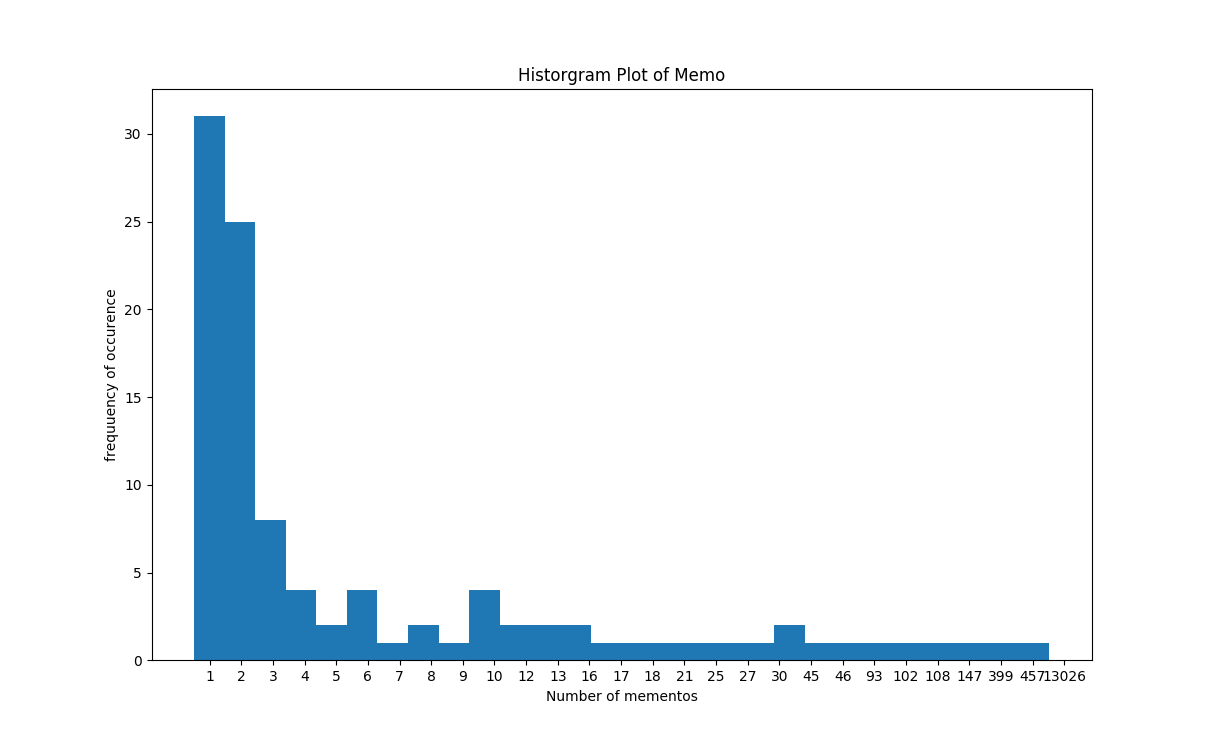
\includegraphics[scale=.5]{histograph.png}
\\
\pagebreak% Create Page break between problems
%----------------------------------------------------------------------------------------
%	Problem 3
%----------------------------------------------------------------------------------------
\section{Problem 3}
\subsection{Question 3}
3.  Estimate the age of each of the 1000 URIs using the "Carbon
Date" tool:\\
\\
http://ws-dl.blogspot.com/2017/09/2017-09-19-carbon-dating-web-version-40.html\\
\\
Note: you should use "docker" and install it locally.  You can do
it like this:\\
\\
http://cd.cs.odu.edu/cd?url=http://www.cs.odu.edu/\\
\\
But it will inevitably crash when everyone tries to use it at the
last minute.\\
\\
For URIs that have > 0 Mementos and an estimated creation date,
create a graph with age (in days) on the x-axis and number of
mementos on the y-axis.\\
\\
Not all URIs will have Mementos, and not all URIs will have an
estimated creation date.  Show how many fall into either categories.
For example,\\
\\
total URIs:         1000\\
no mementos:        137\\
no date estimate:   212\\
\subsection{Answer 3}
Below was the number of links that were submitted to the 
mementos and carbon date websites.\\
\\
Total URIs:			498\\
No mementos:		246\\
No Date Estimate:	0\\
\\
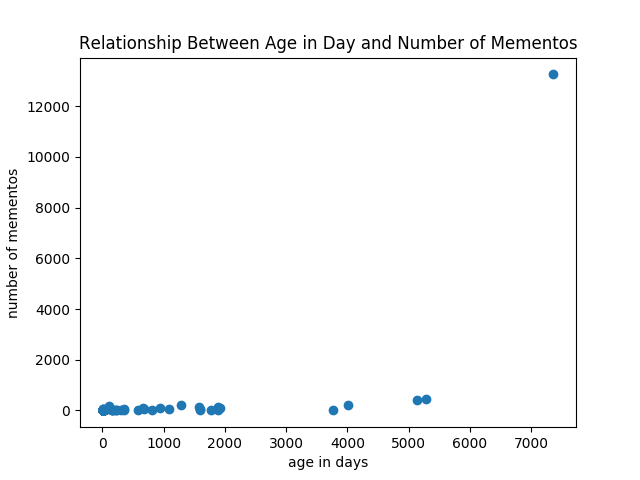
\includegraphics[scale=.5]{scatter.png}


\end{document}
